\documentclass[letterpaper,11pt]{article}

% Soporte para los acentos.
\usepackage[utf8]{inputenc}
\usepackage[T1]{fontenc}
% Idioma español.
\usepackage[spanish,mexico, es-tabla]{babel}
% Soporte de símbolos adicionales (matemáticas)
\usepackage{multirow}
\usepackage{amsmath}
\usepackage{amssymb}
\usepackage{amsthm}
\usepackage{amsfonts}
\usepackage{mathtools}
\usepackage{latexsym}
\usepackage{enumerate}
\usepackage{ragged2e}
\usepackage{listings}
\usepackage[dvipsnames]{xcolor}
\usepackage{graphicx}
\usepackage{hyperref}

% Modificamos los márgenes del documento.                                       
\usepackage[lmargin=1.5cm,rmargin=1.5cm,top=1.5cm,bottom=1.5cm]{geometry}

\title{Complejidad Computacional \\ Tarea 01}
\author{Rubí Rojas Tania Michelle}
\date{\today}

\begin{document}
\maketitle

\begin{enumerate}
    \item Supongamos que un algoritmo $A$, que resuelve un problema $\prod$, 
    tiene un tiempo de ejecución de 
    \begin{equation*}
        T_A(n) = 20n^3 + 10n + 16
    \end{equation*} 
    
    Además, supongamos que un algoritmo $B$, que resuelve el mismo problema 
    $\prod$, tiene un tiempo de ejecución de 
    \begin{equation*}
        T_B(n) = 22n^2 \log_2 (8n)
    \end{equation*} 
    
    ¿Cuál algoritmo es mejor? Justifica tu respuesta respondiendo las 
    siguientes preguntas:
    \begin{enumerate}
        \item ¿Para qué valores de $n$ el algoritmo $A$ es mejor que el $B$.
        \item ¿Para qué valores de $n$ el algoritmo $B$ es mejor que el $A$. 
    \end{enumerate}

    \textsc{Solución:} Inicialmente veamos cómo se comportan estas dos 
    funciones para los primeros $30$ números naturales:
    \begin{figure}[htb]
        \centering
        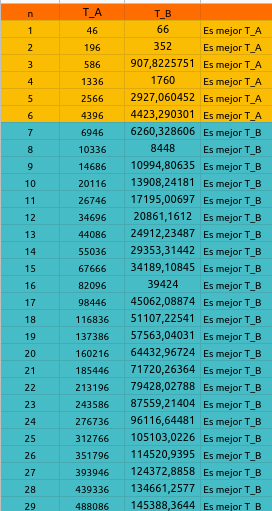
\includegraphics[width=0.31\textwidth]{img/img1.png}
        \caption{Pueden ver la tabla original 
        \href{https://docs.google.com/spreadsheets/d/1dJZr9smxsGQyZ_ItOEklaM7aGh7erAAA3SLIZ5G13YY/edit?usp=sharing}
        {dando click aquí}}
    \end{figure}

    Como podemos observar, cuando $1 \leq n \leq 6$ sucede que el tiempo de 
    ejecución de $T_A$ es menor que el de $T_B$, lo que implica que dentro de 
    este intervalo de valores el algoritmo $A$ es mejor que el $B$. Por otro 
    lado, cuando $n \geq 7$ sucede que el tiempo de ejecución de $T_B$ es menor 
    que el de $T_A$, lo que implica que en ese intervalo de valores el 
    algoritmo $B$ es mejor que el algoritmo $A$. 

    Así que volviendo a la pregunta original, nuestra respuesta sería que el 
    algoritmo $B$ es mejor. Esto se debe al siguiente análisis: El algoritmo 
    $A$ es mejor que el algoritmo $B$ sólo en seis valores de $n$ (donde el 
    número de posibles valores para $n$ es la cardinalidad de $\mathbb{N}$). 
    Si nuestras entradas siempre fueran valores menores o iguales a $6$, 
    entonces claramente la respuesta sería que el algoritmo $A$ es mejor; pero 
    esa condición no la podemos asegurar en ningún caso y como el algoritmo $B$ 
    será el mejor en la mayoría de los casos, entonces nuestra conclusión es que 
    en general el algoritmo $B$ es el mejor. 
\end{enumerate}

\end{document}